\documentclass[12pt]{report}
\usepackage{csvsimple}
\usepackage{graphicx}
\usepackage{float}
\graphicspath{ {images/} }
\usepackage[
backend=bibtex,
style=numeric,
citestyle=numeric,
sorting=none]
{biblatex}
\addbibresource{mybib}
\setlength{\parskip}{5mm}

\begin{document}

\title{OTP and AES: A historical transition between two systems of cryptography}
\author{Valdemar Thanner\\Kantonsschule Zug\\supervised by Mr. Bernhard Keller}
\maketitle

\tableofcontents

\chapter{OTP: The One Time Pad}

\section{What is a "One Time Pad"?}
When speaking about OTP, it is important to distinguish between its two meanings: On the one hand, it is a technique used to encrypt information. This technique requires one single key, used both to encrypt and decrypt the information. This key is also referred to as a one time pad; therefore, it is important to distinguish between the one time pad (a cryptographical technique) and a one time pad (a key which is used to encrypt and decrypt information).

The One Time Pad is largely derived from the Vernam cipher, which is named after Gilbert Vernam. The Vernam cipher utilized a perforated tape (one of the earliest types of data storage) as the secret key\cite{vernampatent}.

\begin{figure}[H]
\centering
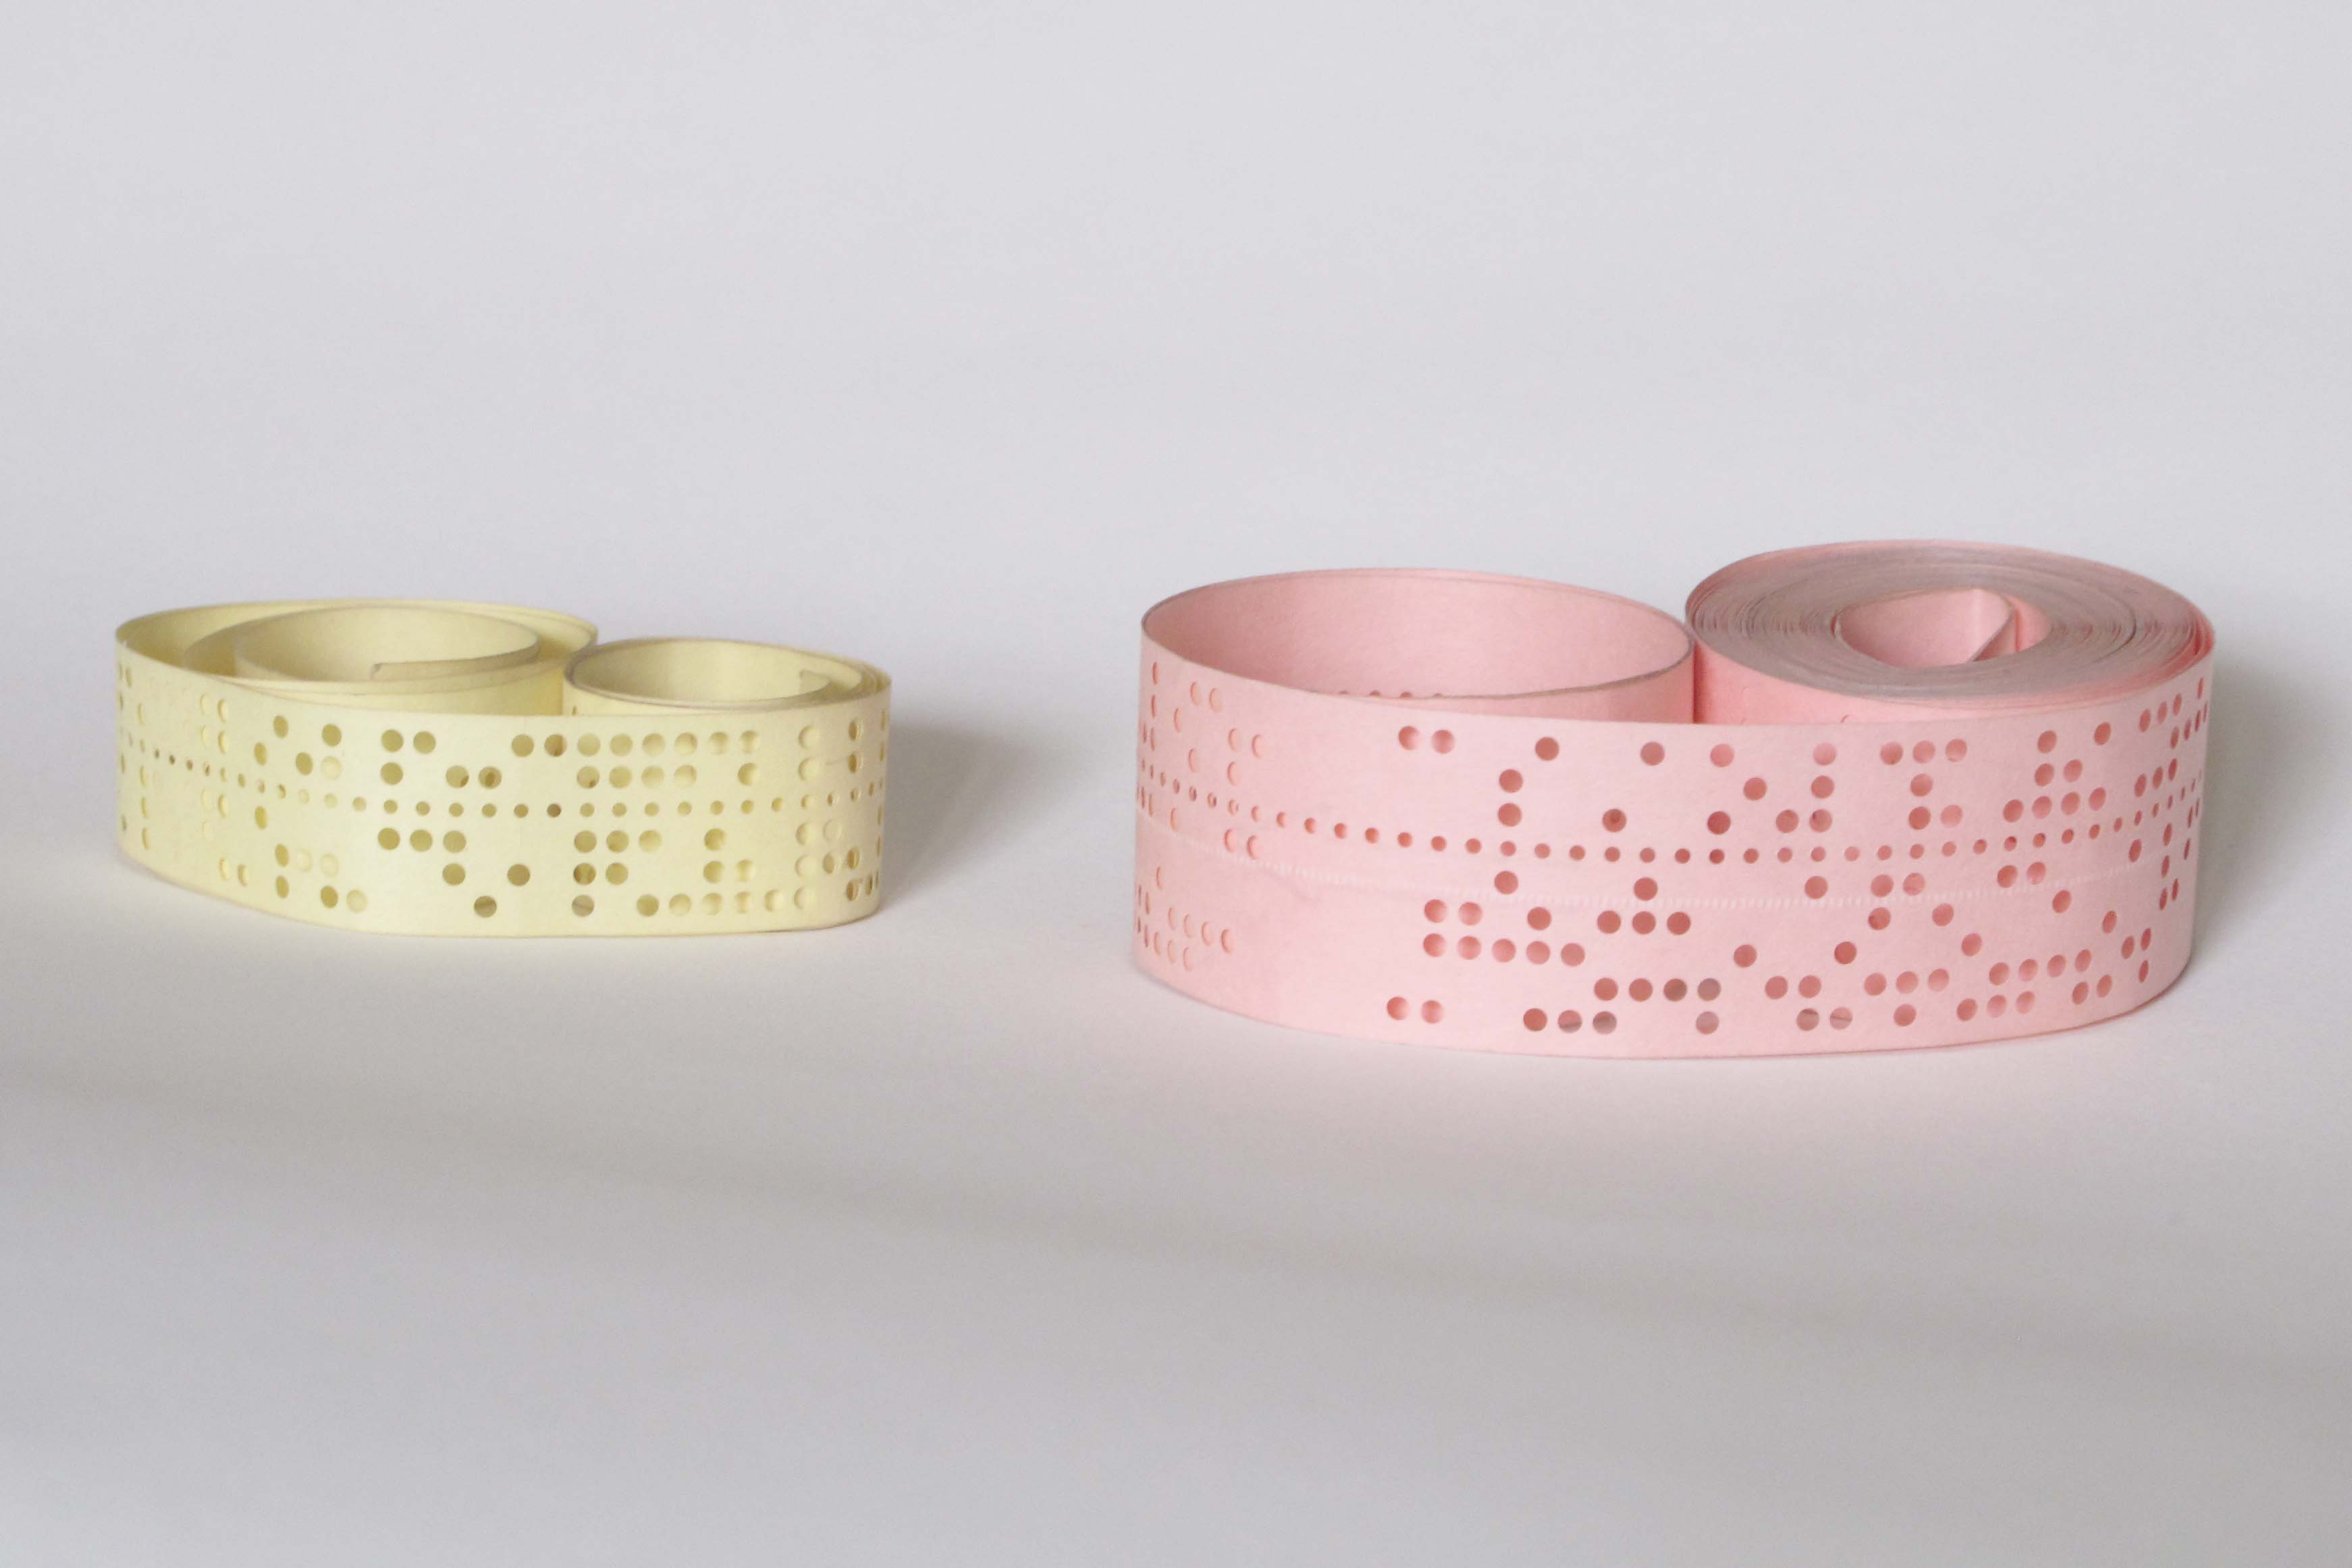
\includegraphics[scale=0.5]{PerforatedTape}
\caption{Perforated tape, utilized to store bits as punched holes}
\end{figure}

However, this system had a vulnerability which the One-Time Pad solved: In Vernam's original method, the perforated tape was not exchanged after it had completed one cycle; instead, it was looped around continuously, often being used multiple times on the same information.    

\section{Method used}

\subsection{Generation of the random key}
In order to encrypt the plaintext, a key must first be generated. This key will be utilized to encrypt the plaintext through the usage of modular addition, turning it into the ciphertext.

This key must fulfil some crucial criteria. Foremost, the length of the key (the amount of  characters contained within it) must be equivalent to or greater than the length of the plaintext; otherwise, it is not possible to perform any encryption (using the OTP). Secondly, the key must be generated randomly. This is mainly due to the fact that a randomly generated key makes frequency analysis\cite{frequencyanalysis}, the form of cryptanalysis most commonly used to break classical ciphers, impossible.

\subsection{Modular addition of the key and plaintext}
Next, the ciphertext is created through modular addition of the key and the plaintext. This can be applied not only to a message consisting of alphabetical characters, but also to any sequence of bits. If the plaintext consists of a message made up of alphabetical characters, the plaintext and the key are added using arithmetic reffered to as \textit{"addition modulo 26"}.

First, each character is assigned a number, in this case corresponding to it's position in the Latin alphabet:

\csvautotabular{tables/ModularAddition.csv}

\subsection{decoding of the ciphertext using the key}

\section{Perfect secrecy: Information-theoretical security}

\subsection{definition}

%\subsection{mathematical proof}

\subsection{Why can only OTP achieve perfect secrecy?}

\section{Issues with OTP}

\subsection{True randomness in generating the key}

\subsection{Secure distribution of the key itself}

\subsection{Secure disposal of a utilized key}


\printbibliography

\end{document}


